\documentclass{beamer}
\mode<presentation>
\usetheme{CambridgeUS}
\usepackage[russian]{babel}
\usepackage[utf8]{inputenc}
\usepackage[T2A]{fontenc}
\usepackage{sansmathaccent}

\usepackage{verbatim}
\usepackage{alltt}

\pdfmapfile{+sansmathaccent.map}
\title[Operating Systems]{Введение в операционные системы}
\author{Наумов Д.А., доц. каф. КТ}
\date[11.02.2019] {Операционные системы и системное программное обеспечение, 2019}

\begin{document}

%ТИТУЛЬНЫЙ СЛАЙД
\begin{frame}
  \titlepage
\end{frame}
  
%СОДЕРЖАНИЕ ЛЕКЦИИ
\begin{frame}
  \frametitle{Содержание лекции}
  \tableofcontents  
\end{frame}

\section{Структура вычислительной системы}
  
\begin{frame}[t]
\begin{block}{Операционная система}
это программа, которая обеспечивает возможность рационального использования оборудования компьютера удобным для пользователя образом. 
\end{block}
Уровни программного обеспечения компьютерной системы
\begin{figure}[h]
\centering
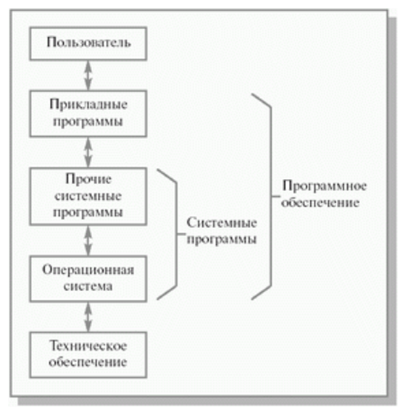
\includegraphics[scale=0.5]{images/lec01-pic01.png}
\label{pic-sort}
\end{figure}
\end{frame} 
   
\section{История развития операционных систем}
   
\begin{frame}[t]
История развития операционных систем
\begin{itemize}
\item 1945-1955 - компьютеры работали без операционных систем
\item 1955-1965 - первые системы пакетной обработки (автоматизировали запуск одной программ за другой и тем самым увеличивали коэффициент загрузки процессора)
\item 1965-1980 - многозадачность (способ организации вычислительного процесса, при котором на одном процессоре попеременно выполняются несколько задач) и система разделения памяти
\item Системы разделения времени - вариант многозадачности, при котором у каждого пользователя есть свой диалоговый терминал (фактически - многопользовательская система)
\item мини-компьютеры (первый - в 1961г.), система MULTICS (предшественник UNIX)
\item разновидности несовместимых UNIX (System V, BSD). Разработка стандарта POSIX (минимальный интерфейс системного вызова, который должны поддерживать системы UNUX).
\end{itemize}
\end{frame} 

\begin{frame}[t]
История развития операционных систем
\begin{itemize}
\item В 1974г. был выпущен центральный процессор Intel 8080, для него была создана операционная система CP/M. В 1977г. она была переработана для других процессоров, например Zilog Z80.
\item В начале 80-х была разработана система MS-DOS, и стала основной системой для микрокомпьютеров.
\item 80-е годы - графический интерфейс пользователя (GUI, Graphical User Interface).
\item С 1985 года стала выпускаться Windows, в то время она была графической оболочкой к MS-DOS вплоть до 1995г., когда вышла Windows 95.
\item IBM и Microsoft начинали совместно разрабатывать операционную систему OS/2. Она должна была поддерживать вытесняющую многозадачность, виртуальную память, графический пользовательский интерфейс, виртуальную машину для выполнения DOS-приложений. Первая версия вышла 1987г.
\item отказ от OS/2 в пользу Windows NT. Первая версия вышла в 1993г.
\end{itemize}
\end{frame} 

\begin{frame}[t]
В середине 80-х стали бурно развиваться сети персональных компьютеров, работающие под управлением сетевых или распределенных операционных систем.
\begin{enumerate}
\item \textbf{Сетевая операционная система} не имеет отличий от операционной системы однопроцессорного компьютера. Она обязательно содержит программную поддержку для сетевых интерфейсных устройств (драйвер сетевого адаптера), а также средства для удаленного входа в другие компьютеры сети и средства доступа к удаленным файлам.
\item \textbf{Распределенная операционная система}, напротив, представляется пользователям простой системой, в которой пользователь не должен беспокоиться о том, где работают его программы или где расположены файлы, все это должно автоматически обрабатываться самой операционной системой.
\end{enumerate}
\begin{itemize}
\item В 1987г. была выпущена операционная система MINIX (прототип LINUX), она была построена на схеме микро ядра.
\item В 1991г. была выпущена LINUX, в отличии от микроядерной MINIX она стала монолитной. Чуть позже вышла FreeBSD (основой для нее послужила BSD UNIX)
\end{itemize}
\end{frame} 

\begin{frame}[t]
\begin{block}{Операционная система как виртуальная машина}
ОС предоставляет пользователю виртуальную машину, которую легче программировать и с которой легче работать, чем непосредственно с аппаратурой, составляющей реальную машину. 
\end{block}
\end{frame}

\begin{frame}[t]
\begin{block}{Операционная система как менеджер ресурсов}
Чтобы несколько программ могло работать с одним ресурсом (процессор, память), необходима система управления ресурсами. 
\end{block}
Способы распределения ресурса:
\begin{itemize}
\item Временной - когда программы используют его по очереди, например, так система управляет процессором.
\item Пространственный - программа получает часть ресурса, например, так система управляет оперативной памятью и жестким диском.
\end{itemize}
\end{frame}

\section{Основные понятия, концепции ОС}
\begin{frame}[t]
\begin{block}{Системные вызовы (system calls)}
это интерфейс между операционной системой и пользовательской программой. Они создают, удаляют и используют различные объекты, главные из которых – процессы и файлы. Пользовательская программа запрашивает сервис у операционной системы, осуществляя системный вызов.  
\end{block}
При системном вызове задача переходит в привилегированный режим или режим ядра (kernel mode). Поэтому системные вызовы иногда еще называют программными прерываниями, в отличие от аппаратных прерываний, которые чаще называют просто прерываниями.

В большинстве операционных систем системный вызов осуществляется командой программного прерывания (INT). Программное прерывание – это синхронное событие, которое может быть повторено при выполнении одного и того же программного кода.
\end{frame}

\begin{frame}[t]
\begin{block}{Интерфейс прикладного программирования, API (Application Programming Interface)}
интерфейс между операционной системой и программами, определяемый набором системных вызовов.
\end{block}
Некоторые системные вызовы в POSIX:
\begin{itemize}
\item fork - создание нового процесса
\item exit - завершение процесса
\item open - открывает файл
\item close - закрывает файл
\item read - читает данные из файла в буфер
\item write - пишет данные из буфера в файл
\end{itemize}
В UNIX вызовы почти один к одному идентичны библиотечным процедурам, которые используются для обращения к системным вызовам.
\end{frame}

\begin{frame}[t]
Win32 API отделен от системных вызовов. Это позволяет в разных версиях менять системные вызовы, не переписывая программы. Поэтому непонятно является ли вызов системным (выполняется ядром), или он обрабатывается в пространстве пользователя.

Некоторые системные вызовы в Windows (Win32 API):
\begin{itemize}
\item CreatProcess (fork) - создание нового процесса
\item ExitProcess (exit) - завершение процесса
\item CreatFile (open) - открывает файл
\item CloseHandle (close) - закрывает файл
\end{itemize}
В Win32 API существует более 1000 вызовов. Такое количество связано и с тем, что графический интерфейс пользователя UNIX запускается в пользовательском режиме, а в Windows встроен в ядро. Поэтому Win32 API имеет много вызовов для управления окнами, текстом, шрифтами т.д.
\end{frame}

\begin{frame}[t]
\begin{block}{Прерывание (hardware interrupt)}
это событие, генерируемое внешним (по отношению к процессору) устройством.
\end{block}
\begin{itemize}
\item важный тип аппаратных прерываний – прерывания таймера, которые генерируются периодически через фиксированный промежуток времени. Прерывания таймера используются операционной системой при планировании процессов. 
\item Каждый тип аппаратных прерываний имеет собственный номер, однозначно определяющий источник прерывания.
\item Аппаратное прерывание – это асинхронное событие, то есть оно возникает вне зависимости от того, какой код исполняется процессором в данный момент. 
\item Обработка аппаратного прерывания не должна учитывать, какой процесс является текущим.
\end{itemize}
\end{frame}

\begin{frame}[t]
\begin{block}{Исключительная ситуация (exception)}
событие, возникающее в результате попытки выполнения программой команды, которая по каким-то причинам не может быть выполнена до конца.
\end{block}
Исключительные ситуации, как и системные вызовы, являются синхронными событиями, возникающими в контексте текущей задачи. 
\begin{itemize}
\item исправимые (например, отсутствие информации в памяти)
\item неисправимые (деление на ноль)
\end{itemize}
\end{frame}

\begin{frame}[t]
\begin{block}{Файл}
(обычно) именованная часть пространства на носителе информации.
\end{block}
Главная задача файловой системы (file system) – скрыть особенности ввода-вывода и дать программисту простую абстрактную модель файлов, независимых от устройств. 
\begin{block}{Процессы, нити}
наиболее фундаментальные понятия, будут рассмотрены далее
\end{block}
\end{frame}

\section{Архитектурные особенности ОС}

\begin{frame}[t]
Система с монолитным ядром
\begin{figure}[h]
\centering
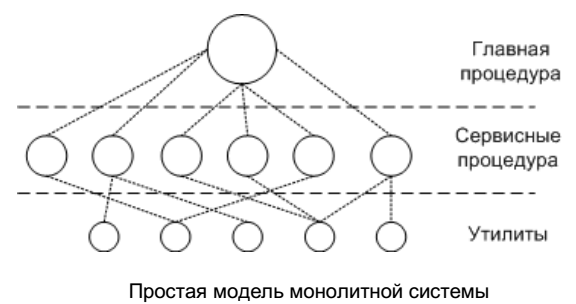
\includegraphics[scale=0.5]{images/lec01-pic02.png}
\end{figure}
\begin{itemize}
\item главная программа, которая вызывает требуемые сервисные процедуры.
\item набор сервисных процедур, реализующих системные вызовы
\item набор утилит, обслуживающих сервисные процедуры
\end{itemize}
\end{frame}

\begin{frame}[t]
Для каждого системного вызова имеется одна сервисная процедура. Утилиты выполняют функции, которые нужны нескольким сервисным процедурам.
\begin{figure}[h]
\centering
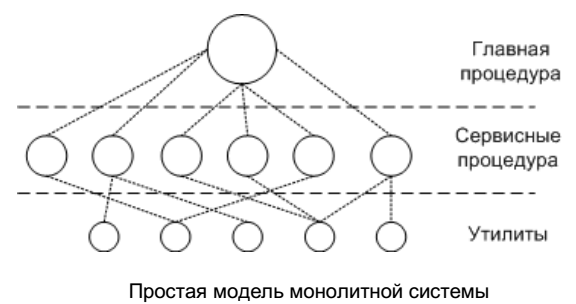
\includegraphics[scale=0.4]{images/lec01-pic02.png}
\end{figure}
Этапы обработки вызова:
\begin{itemize}
\item Принимается вызов
\item Выполняется переход из режима пользователя в режим ядра
\item ОС проверяет параметры вызова для того, чтобы определить, какой системный вызов должен быть выполнен
\item После этого ОС обращается к таблице, содержащей ссылки на процедуры, и вызывает соответствующую процедуру
\end{itemize}
\end{frame}

\begin{frame}[t]
Многоуровневые системы
\begin{figure}[h]
\centering
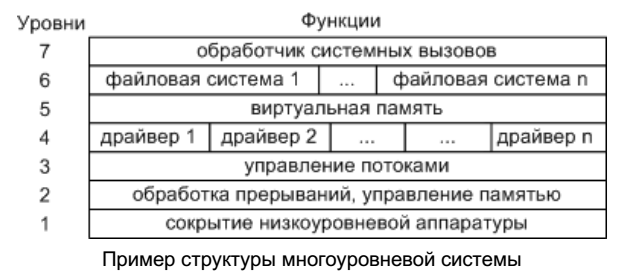
\includegraphics[scale=0.5]{images/lec01-pic03.png}
\end{figure}
Обобщением предыдущего подхода является организация ОС как иерархии уровней. 
\begin{itemize}
\item уровни образуются группами функций операционной системы - файловая система, управление процессами и устройствами и т.п. 
\item Каждый уровень может взаимодействовать только со своим непосредственным соседом - выше- или нижележащим уровнем. 
\item Прикладные программы или модули самой операционной системы передают запросы вверх и вниз по этим уровням.
\end{itemize}
\end{frame}

\begin{frame}[t]
Многоуровневые системы
\begin{figure}[h]
\centering
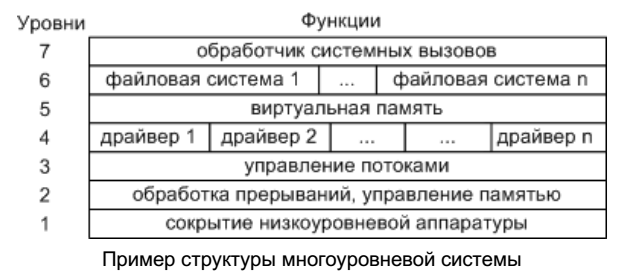
\includegraphics[scale=0.6]{images/lec01-pic03.png}
\end{figure}
Преимущества 
\begin{itemize}
\item Высокая производительность
\end{itemize}
Недостатки 
\begin{itemize}
\item Большой код ядра, и как следствие большое содержание ошибок
\item Ядро плохо защищено от вспомогательных процессов
\end{itemize}
\end{frame}

\begin{frame}[t]
Пример многоуровневой структуры OS UNIX
\begin{figure}[h]
\centering
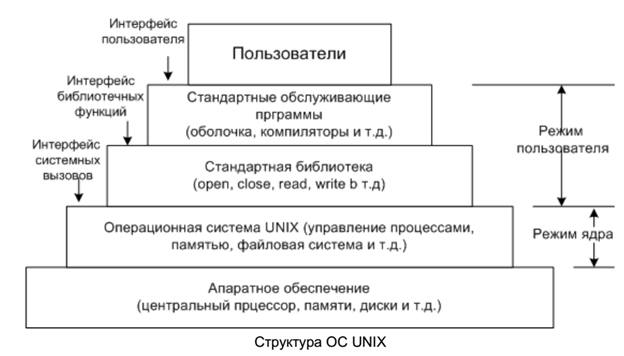
\includegraphics[scale=0.7]{images/lec01-pic04.png}
\end{figure}
\end{frame}

\begin{frame}[t]
Пример структуры OS Windows NT
\begin{figure}[h]
\centering
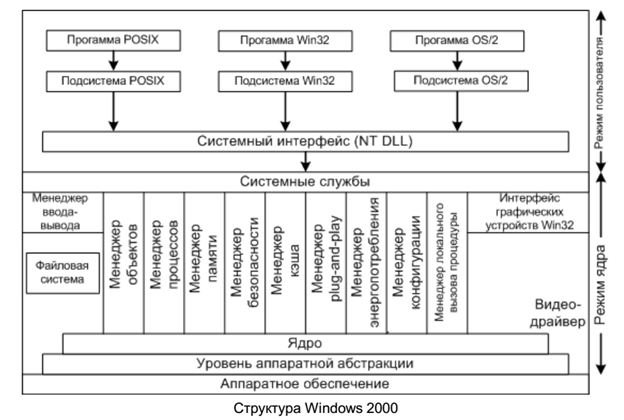
\includegraphics[scale=0.7]{images/lec01-pic05.png}
\end{figure}
\end{frame}

\begin{frame}[t]
Модель экзоядра

Принцип экзоядра: все отдать пользовательским программам. 

Например, зачем нужна файловая система? 
\begin{itemize}
\item каждая пользовательская программа сможет иметь свою файловую систему.
\item операционная система должна обеспечить безопасное распределение ресурсов среди соревнующихся за них пользователей.
\end{itemize}
\end{frame}

\begin{frame}[t]
Микроядерная архитектура (Эта модель является средним между двумя предыдущими моделями)
\begin{figure}[h]
\centering
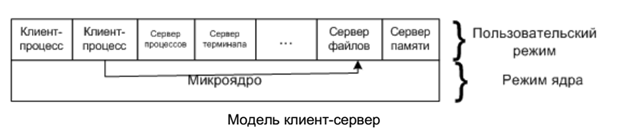
\includegraphics[scale=0.75]{images/lec01-pic06.png}
\end{figure}
В этой модели вводятся два понятия:
\begin{itemize}
\item Серверный процесс (который обрабатывает запросы)
\item Клиентский процесс (который посылает запросы)
\end{itemize}
Недостатки 
В задачу ядра входит только управление связью между клиентами и серверами.
\end{frame}

\begin{frame}[t]
Микроядерная архитектура (Эта модель является средним между двумя предыдущими моделями)
\begin{figure}[h]
\centering
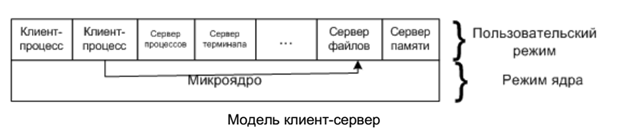
\includegraphics[scale=0.75]{images/lec01-pic06.png}
\end{figure}
Преимущества
\begin{itemize}
\item Малый код ядра и отдельных подсистем, и как следствие меньшее содержание ошибок.
\item Ядро лучше защищено от вспомогательных процессов.
\item Легко адаптируется к использованию в распределенной системе
\end{itemize}
Недостатки 
\begin{itemize}
\item Уменьшение производительности.
\end{itemize}
\end{frame}

\begin{frame}[t]
Сравнение моделей
\begin{figure}[h]
\centering
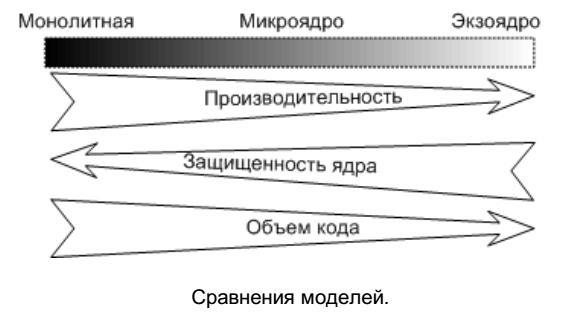
\includegraphics[scale=0.75]{images/lec01-pic07.png}
\end{figure}
\end{frame}

\end{document}
